\section{Matrix-based multiple-source CFPQ algorithm}
\label{sec:multiple-source-algo}

 In this section we introduce two versions of the multiple-source matrix-based CFPQ algorithm.
 This algorithm is a modification of Azimov's matrix-based algorithm for CFPQ and its core idea is to cut off those vertices which are not in the selected set of start vertices.


In order to simplify Azimov's algorithm modification and the final algorithm description, we assume the input graph to have only edge labels.
Note, that we always can convert the original graph into such form.
To do it, we should add loops into vertices in the following way: for the vertex $i$ we add an edge $i \xrightarrow{x} i$ iff $\lambda_V(i) = x$ and $x\neq \varnothing$.
This way we can switch to an edge-labeled graph with the same number of vertices while preserving the defined semantics of CFPQ.

\begin{figure}[h]
    \centering
    \begin{tikzpicture}[shorten >=1pt,auto]
       \node[state] (q_0)                        {$0$};
       \node[state] (q_1) [right=of q_0]         {$1$};
       \node[state] (q_2) [below left=of q_1]    {$2$};
       \node[state] (q_3) [below left=of q_2]    {$3$};
       \node[state] (q_4) [below right=of q_2]   {$4$};
       \node[state] (q_5) [below right=of q_1]   {$5$};
       \path[->]
        (q_0) edge[loop left]  node {$\{x, y\}$} (q_0)
        (q_0) edge  node {$\{a\}$} (q_1)
        (q_2) edge[loop left]  node {$\{x\}$} (q_2)
        (q_1) edge  node {$\{b\}$} (q_5)
        (q_1) edge  node {$\{a, b\}$} (q_2)
        (q_3) edge[above]  node {$\{c\}$} (q_2)
        (q_4) edge  node {$\{c\}$} (q_3)
        (q_2) edge[above]  node {$\{c\}$} (q_4)
        (q_4) edge[loop below]  node {$\{y\}$} (q_4)
        (q_5) edge[bend left, below]  node {$\{d\}$} (q_4)
        (q_4) edge[bend left, above]  node {$\{d\}$} (q_5);
    \end{tikzpicture}
    \caption{The example of $D_1'$: the modified input graph $D_1$}
    \label{fig:example_modified_input_graph}
\end{figure}

The adjacency matrix $M$ of the graph $D_1'$ is
{
    \renewcommand{\arraystretch}{0.7}
    \setlength\arraycolsep{2pt}
$$
    M =
    \begin{pmatrix}
    \{x, y\}     & \{a\}       & \varnothing & \varnothing & \varnothing & \varnothing \\
    \varnothing  & \varnothing & \{a, b\}    & \varnothing & \varnothing & \{b\}       \\
    \varnothing  & \varnothing & \{x\}       & \varnothing & \{c\}       & \varnothing \\
    \varnothing  & \varnothing & \{c\}       & \varnothing & \varnothing & \varnothing \\
    \varnothing  & \varnothing & \varnothing & \{c\}       & \{y\}       & \{d\}       \\
    \varnothing  & \varnothing & \varnothing & \varnothing & \{d\}       & \varnothing
    \end{pmatrix}.
$$
}
Note that this transformation is impractical for real-world graphs, thus we use it only for algorithm description.

The first version of multiple-source algorithm is the Azimov's algorithm equipped with vertices filtering.
Let $G = (N, \Sigma, P, S)$ be the input context-free grammar, $D = (V, E, \Sigma_V, \Sigma_E, \lambda_V, \lambda_E)$ be the input graph and $Src$ be the input set of start vertices.
The result of the algorithm is a Boolean matrix which represents relation $R_{S,D}^{Src}$.

\begin{algorithm}
\begin{algorithmic}[1]
\caption{Multiple-source context-free path querying algorithm}
\label{alg:algo1}
\Function{MultiSrcCFPQ}{\par
\hskip\algorithmicindent $D = (V, E, \Sigma_V, \Sigma_E, \lambda_V, \lambda_E)$, \par
\hskip\algorithmicindent $G=(N,\Sigma,P,S)$, \par
\hskip\algorithmicindent
$Src$}
    \State{$T \gets \{T^A \mid  A \in N, T^A_{i,j} \gets \textit{false} \text{, for all $i,j$}\} $}

    \State{$TSrc \gets \{TSrc^A \mid  A \in N, TSrc^A_{i,j} \gets \textit{false} \text{, for all $i,j$}\}$}

    \ForAll{$ v \in Src$} \Comment{Input matrix initialization}
        \State{$TSrc^S_{v,v} \gets true$}
    \EndFor

    \ForAll{$A \to x \in P$} \Comment{Simple rules initialization}
        \ForAll{$(v, to) \in E, \lambda_E(v,to) = x$}
            \State{$T^A_{v,to} \gets true$}
        \EndFor
    \EndFor

    \While{$T\ or\ TSrc\ is\ changing$} \Comment{Algorithm's body}
        \ForAll{$A \to B C \in P$}
            \State{$M \gets TSrc^A*T^B$}
            \State{$T^A \gets T^A + M*T^C$}
            \State{$TSrc^B \gets TSrc^B + TSrc^A$}
            \State{$TSrc^C \gets TSrc^C + $ \Call{getDst}{$M$}}
        \EndFor
    \EndWhile
    \State \Return $T^S$
\EndFunction



\Function{getDst}{$M$}
    \State{$A_{i,j} \gets \textit{false}$}
    \ForAll{$(v,to) \in V^2 \mid M_{v,to} = true$}
        \State{$A_{to,to} \gets true$}
    \EndFor
    \State \Return A
\EndFunction
\end{algorithmic}
\end{algorithm}

In order to solve the single-source and multiple-source CFPQ problem, we modified the Azimov's algorithm.
Each time, when a grammar rule is applied (see line \textbf{8} of Algorithm~\ref{alg:algo0}: boolean matrix multiplication $T_A = T_A + T_B \cdot T_C$ for each $A \rightarrow BC \in P$), only vertices of interest should be stored.
To do it, we added one more matrix multiplication: $T_A = T_A + (TSrc^A \cdot T_B) \cdot T_C$, where $TSrc^A$ --- matrix of start vertices for the current iteration (lines \textbf{11-13} of the Algorithm~\ref{alg:algo1}).
After every iteration of the while loop, it is necessary to update the set of vertices paths from which we need to calculate.
To do it, the we call the function \textsc{getDst} (see lines \textbf{17-21}), in line \textbf{14}.
Thus, the modified algorithm supports the frontier of the vertices of interest and updates it on each iteration.
As a result, it only computes the paths which starts from the small set of selected vertices.

In case when one has a sequence of similar queries to the single graph, it may be useful to cache results of the query evaluation and share them between queries.
This may help to avoid recalculation of the already computed results.
To introduce \cho{interqueries} caching, we modify the previous version of the algorithm.
The modified version stores all the vertices the paths from which have already been calculated in cache \textit{index}, which is used to filter such vertices in line \textbf{11} of Algorithm~\ref{alg:algo2}.
Thus, the modified algorithm calculates paths from the particular vertex only once.
Note, that \textsc{CreateIndex} function should be called first, and the created index can be shared between multiple calls of \textsc{MultiSrcCFPQSmart} after that.

\begin{algorithm}
\begin{algorithmic}[1]
\caption{Optimized multiple-source context-free path querying algorithm}
\label{alg:algo2}
\Function{CreateIndex}{ \par
\hskip\algorithmicindent $D = (V, E, \Sigma_V, \Sigma_E, \lambda_V, \lambda_E)$, \par
\hskip\algorithmicindent $G=(N,\Sigma,P,S)$}
    \State{$T \gets \{T^A \mid  A \in N, T^A_{i,j} \gets \textit{false} \text{, for all $i,j$}\}$}

    \State{$TSrc \gets \{TSrc^A \mid  A \in N, TSrc^A_{i,j} \textit{false} \text{, for all $i,j$}\}$}

    \ForAll{$A \to x \in P$} \Comment{Simple rules initialization}
        \ForAll{$(v, to) \in E, \lambda_E(v,to) = x$}
            \State{$T^A_{v,to} \gets true$}
        \EndFor
    \EndFor

    \State \Return $(T, TSrc)$
\EndFunction
\State
\Function{MultiSrcCFPQSmart}{ \par
\hskip\algorithmicindent $D = (V, E, \Sigma_V, \Sigma_E, \lambda_V, \lambda_E)$, \par
\hskip\algorithmicindent $G=(N,\Sigma,P,S)$, \par
\hskip\algorithmicindent $Src$, \par
\hskip\algorithmicindent $Index = (T, TSrc)$}

    \State{$TNewSrc \gets \{TNewSrc^A \mid  A \in N, TNewSrc^A \gets \varnothing\}$}

    \ForAll{$v \in Src \mid TSrc_{v,v} = false$}
        \State{$TNewSrc^S_{v,v} \gets true$}
    \EndFor

    \While{\textit{T or TNewSrc is changing}}
        \ForAll{$A \to B C \in P$}
            \State{$M \gets TNewSrc^A*T^B$}
            \State{$T^A \gets T^A + M*T^C$}

            \State{$TNewSrc^B \gets TNewSrc^B + TNewSrc^A \setminus TSrc^B$}
            \State{$TNewSrc^C \gets TNewSrc^C + $ \Call{getDst}{M}} $\setminus$ $TSrc^C$
        \EndFor
    \EndWhile
    \Return{$ TSrc^S*T^S $}
    \Comment{We want to return only relevant data, not all cached results}
\EndFunction


\end{algorithmic}
\end{algorithm}


\subsection{Example}

Consider the first few steps of the proposed algorithm (without caching) on the graph $D_1'$, grammar $G_1^{\text{wcnf}}$, and the set of start vertices $Src = \{2\}$.
At the first step (lines \textbf{4}--\textbf{5}) $TSrc^S_{2,2}$ sets to \textit{true}, all other cells have value \textit{false}.
Then the set of matrices $T$ is initialized using rules $C \to c, D \to d, Y \to y$ as follows:
{
    \renewcommand{\arraystretch}{0.7}
    \setlength\arraycolsep{2pt}
\begin{align*}
    T^C& = \mathcal{E}^c =
    \begin{pmatrix}
    . & . & . & . & . & . \\
    . & . & . & . & . & . \\
    . & . & . & . & 1 & . \\
    . & . & 1 & . & . & . \\
    . & . & . & 1 & . & . \\
    . & . & . & . & . & .
\end{pmatrix},
    T^D = \mathcal{E}^d =
    \begin{pmatrix}
    . & . & . & . & . & . \\
    . & . & . & . & . & . \\
    . & . & . & . & . & . \\
    . & . & . & . & . & . \\
    . & . & . & . & . & 1 \\
    . & . & . & . & 1 & .
\end{pmatrix},\\
    T^Y& = \mathcal{V}^y =
    \begin{pmatrix}
    1 & . & . & . & . & . \\
    . & . & . & . & . & . \\
    . & . & . & . & . & . \\
    . & . & . & . & . & . \\
    . & . & . & . & 1 & . \\
    . & . & . & . & . & .
\end{pmatrix}
\end{align*}
}

The following computations take place at the first iteration of the while loop in line~\textbf{9} for the grammar rule $S \to C E$.
First, the matrix $M$ is computed as follows
{
    \renewcommand{\arraystretch}{0.7}
    \setlength\arraycolsep{2pt}
\begin{align*}
M=TSrc^S*T^C =
\begin{pmatrix}
    . & . & . & . & . & . \\
    . & . & . & . & . & . \\
    . & . & 1 & . & . & . \\
    . & . & . & . & . & . \\
    . & . & . & . & . & . \\
    . & . & . & . & . & .
\end{pmatrix}*
\begin{pmatrix}
    . & . & . & . & . & . \\
    . & . & . & . & . & . \\
    . & . & . & . & 1 & . \\
    . & . & 1 & . & . & . \\
    . & . & . & 1 & . & . \\
    . & . & . & . & . & .
\end{pmatrix}=
\begin{pmatrix}
    . & . & . & . & . & . \\
    . & . & . & . & . & . \\
    . & . & . & . & 1 & . \\
    . & . & . & . & . & . \\
    . & . & . & . & . & . \\
    . & . & . & . & . & .
\end{pmatrix}
\end{align*}
}

Since matrix $T^E$ is empty, $T^S$ stays the same in line~\textbf{12}, as well as $TSrc^C$ in line~\textbf{13}.
But the matrix $TSrc^E$ is updated (line~\textbf{14}):
{
    \renewcommand{\arraystretch}{0.7}
    \setlength\arraycolsep{2pt}
\begin{align*}
&TSrc^E = TSrc^E + \textsc{getDist}(M) = \\ &=
\begin{pmatrix}
    . & . & . & . & . & . \\
    . & . & . & . & . & . \\
    . & . & . & . & . & . \\
    . & . & . & . & . & . \\
    . & . & . & . & . & . \\
    . & . & . & . & . & .
\end{pmatrix} +
\begin{pmatrix}
    . & . & . & . & . & . \\
    . & . & . & . & . & . \\
    . & . & . & . & . & . \\
    . & . & . & . & . & . \\
    . & . & . & . & 1 & . \\
    . & . & . & . & . & .
\end{pmatrix}=
\begin{pmatrix}
    . & . & . & . & . & . \\
    . & . & . & . & . & . \\
    . & . & . & . & . & . \\
    . & . & . & . & . & . \\
    . & . & . & . & 1 & . \\
    . & . & . & . & . & .
\end{pmatrix}
\end{align*}
}

This means that we are interested in paths that start from the vertex 4 and satisfy the constraints specified by nonterminal $E$.

The second rule is $S \to C S_1$ and its processing is similar to previous one.
After processing,
{
    \renewcommand{\arraystretch}{0.7}
    \setlength\arraycolsep{2pt}
\begin{align*}
TSrc^{S_1} =
\begin{pmatrix}
    . & . & . & . & . & . \\
    . & . & . & . & . & . \\
    . & . & . & . & . & . \\
    . & . & . & . & . & . \\
    . & . & . & . & 1 & . \\
    . & . & . & . & . & .
\end{pmatrix},
\end{align*}
}

The third rule is $E \to Y D$.
Here $M$ is computed as follows:
{
    \renewcommand{\arraystretch}{0.7}
    \setlength\arraycolsep{2pt}
\begin{align*}
M = TSrc^E * T^Y =
\begin{pmatrix}
    . & . & . & . & . & . \\
    . & . & . & . & . & . \\
    . & . & . & . & . & . \\
    . & . & . & . & . & . \\
    . & . & . & . & 1 & . \\
    . & . & . & . & . & .
\end{pmatrix}*
\begin{pmatrix}
    1 & . & . & . & . & . \\
    . & . & . & . & . & . \\
    . & . & . & . & . & . \\
    . & . & . & . & . & . \\
    . & . & . & . & 1 & . \\
    . & . & . & . & . & .
\end{pmatrix}=
\begin{pmatrix}
    . & . & . & . & . & . \\
    . & . & . & . & . & . \\
    . & . & . & . & . & . \\
    . & . & . & . & . & . \\
    . & . & . & . & 1 & . \\
    . & . & . & . & . & .
\end{pmatrix}
\end{align*}
}

Then the algorithm updates $T^E$ as follows:

{
    \renewcommand{\arraystretch}{0.7}
    \setlength\arraycolsep{2pt}
\begin{align*}
&T^E = T^E + M * T^D = \\ &=
\begin{pmatrix}
    . & . & . & . & . & . \\
    . & . & . & . & . & . \\
    . & . & . & . & . & . \\
    . & . & . & . & . & . \\
    . & . & . & . & . & . \\
    . & . & . & . & . & .
\end{pmatrix}+
\begin{pmatrix}
    . & . & . & . & . & . \\
    . & . & . & . & . & . \\
    . & . & . & . & . & . \\
    . & . & . & . & . & . \\
    . & . & . & . & 1 & . \\
    . & . & . & . & . & .
\end{pmatrix}*
\begin{pmatrix}
    . & . & . & . & . & . \\
    . & . & . & . & . & . \\
    . & . & . & . & . & . \\
    . & . & . & . & . & . \\
    . & . & . & . & . & 1 \\
    . & . & . & . & 1 & .
\end{pmatrix}=
\begin{pmatrix}
    . & . & . & . & . & . \\
    . & . & . & . & . & . \\
    . & . & . & . & . & . \\
    . & . & . & . & . & . \\
    . & . & . & . & . & 1 \\
    . & . & . & . & . & .
\end{pmatrix}
\end{align*}
}

Thus we know that there exists a path from vertex 4 to vertex 5 such that it forms a word derivable from $E$.

The last rule is $S_1 \to S D$.
During processing this rule only $TSrc^S$ is updated, since $T^S$ is empty:
{
    \renewcommand{\arraystretch}{0.7}
    \setlength\arraycolsep{2pt}
\begin{align*}
&TSrc^S = TSrc^S + TSrc^{S_1} = \\ &=
\begin{pmatrix}
    . & . & . & . & . & . \\
    . & . & . & . & . & . \\
    . & . & 1 & . & . & . \\
    . & . & . & . & . & . \\
    . & . & . & . & . & . \\
    . & . & . & . & . & .
\end{pmatrix}*
\begin{pmatrix}
    . & . & . & . & . & . \\
    . & . & . & . & . & . \\
    . & . & . & . & . & . \\
    . & . & . & . & . & . \\
    . & . & . & . & 1 & . \\
    . & . & . & . & . & .
\end{pmatrix}=
\begin{pmatrix}
    . & . & . & . & . & . \\
    . & . & . & . & . & . \\
    . & . & 1 & . & . & . \\
    . & . & . & . & . & . \\
    . & . & . & . & 1 & . \\
    . & . & . & . & . & .
\end{pmatrix}
\end{align*}
}

This is the end of the first iteration.

At the second iteration, matrices $M$ and then $T^S$ are computed for rule $S \to C E$ as follows:
{
    \renewcommand{\arraystretch}{0.7}
    \setlength\arraycolsep{2pt}
\begin{align*}
&M = TSrc^S * T^C =
\begin{pmatrix}
    . & . & . & . & . & . \\
    . & . & . & . & . & . \\
    . & . & 1 & . & . & . \\
    . & . & . & . & . & . \\
    . & . & . & . & 1 & . \\
    . & . & . & . & . & .
\end{pmatrix} *
\begin{pmatrix}
    . & . & . & . & . & . \\
    . & . & . & . & . & . \\
    . & . & . & . & 1 & . \\
    . & . & 1 & . & . & . \\
    . & . & . & 1 & . & . \\
    . & . & . & . & . & .
\end{pmatrix}=
\begin{pmatrix}
    . & . & . & . & . & . \\
    . & . & . & . & . & . \\
    . & . & . & . & 1 & . \\
    . & . & . & . & . & . \\
    . & . & . & 1 & . & . \\
    . & . & . & . & . & .
\end{pmatrix}
\\
&T^S = M * T^E =
\begin{pmatrix}
    . & . & . & . & . & . \\
    . & . & . & . & . & . \\
    . & . & . & . & 1 & . \\
    . & . & . & . & . & . \\
    . & . & . & 1 & . & . \\
    . & . & . & . & . & .
\end{pmatrix} *
\begin{pmatrix}
    . & . & . & . & . & . \\
    . & . & . & . & . & . \\
    . & . & . & . & . & . \\
    . & . & . & . & . & . \\
    . & . & . & . & . & 1 \\
    . & . & . & . & . & .
\end{pmatrix} =
\begin{pmatrix}
    . & . & . & . & . & . \\
    . & . & . & . & . & 1 \\
    . & . & . & . & . & . \\
    . & . & . & . & . & . \\
    . & . & . & . & . & . \\
    . & . & . & . & . & .
\end{pmatrix}
\end{align*}
}

Thus, we found the first path that satisfies our query.
After all iterations finished, we get the final result:
{
    \renewcommand{\arraystretch}{0.7}
    \setlength\arraycolsep{2pt}
\begin{align*}
T^S =
\begin{pmatrix}
    . & . & . & . & . & . \\
    . & . & . & . & 1 & 1 \\
    . & . & . & . & . & . \\
    . & . & . & . & . & . \\
    . & . & . & . & . & . \\
    . & . & . & . & . & .
\end{pmatrix}
\end{align*}
}
Thus only vertices 4 and 5 are reachable from the vertex 2 by a path which forms a word derivable from the start nonterminal $S$.

\subsection{Implementation Notes}

All of the versions presented have been implemented$\footnote{GitHub repository with implemented algorithms: \url{https://github.com/JetBrains-Research/CFPQ_PyAlgo}, last accessed 28.08.2020}$ using GraphBLAS framework that allows one to represent graphs as matrices and to work with them in terms of linear algebra.
For~convenience, the code is written in Python using pygraphblas\footnote{GitHub repository of PyGraphBLAS library: \url{https://github.com/michelp/pygraphblas}}, which is a Python wrapper for GraphBLAS API and is based on SuiteSparse:GraphBLAS\footnote{GitHub repository of SuiteSparse:GraphBLAS library: \url{https://github.com/DrTimothyAldenDavis/SuiteSparse}}~\cite{10.1145/3322125} --- the complete implementation of the GraphBLAS standard.
This library is specialized to work with sparse matrices which appear in real graphs most often.
% Relevance?
\cho{It should be noted that, despite the fact that the function \textsc{getDst} does not seem to be expressed in terms of linear algebra, the implementation employs the function \textsc{reduce\_vector} from pygraphblas.}

\subsection{Algorithm Evaluation}\label{sect:py_algo_evaluation}

We evaluate both described versions of the multiple-source algorithm on real-world graphs.
For evaluation, we use a PC with Ubuntu 20.04 installed.
It has Intel core i7-4790 CPU, 3.60GHz, and DDR3 32Gb RAM.
As far as we evaluate only the execution time of the algorithm, we store each graph fully in RAM as its adjacency matrix in sparse format.
Note, that graph loading time is not included in the result time of evaluation.

For evaluation we use graphs and queries from CFPQ\_Data dataset\footnote{CFPQ\_Data is a dataset for CFPQ evaluation which contains both synthetic and real-world data and queries \url{https://github.com/JetBrains-Research/CFPQ\_Data}, last accessed 28.08.2020.}
Detailed information, such as the number of vertices and edges, and the number of edges with the specific label, on graphs used in evaluation is provided in table~\ref{tbl:graphs_for_cfpq}.
We use classical same-generation queries $g_1$~(eq.~\ref{eqn:g_1}) and $g_2$~(eq.~\ref{eqn:g_2}) which are used in other works for CFPQ evaluation.
We also use $geo$~(eq.~\ref{eqn:geo}) query provided by \cho{J. Kuijpers} et. al~\cite{Kuijpers:2019:ESC:3335783.3335791} for \textit{geospecies} RDF.
Note that in queries we use $\overline{x}$ notation to denote the inverse of the $x$ relation and the respective edge.

\begin{align}
\begin{split}
\label{eqn:g_1}
S \to & \overline{\textit{subClassOf}} \ \ S \ \textit{subClasOf} \mid \overline{\textit{type}} \ \ S \ \textit{type}\\   & \mid \overline{\textit{subClassOf}} \ \ \textit{subClasOf} \mid \overline{\textit{type}} \ \textit{type}
\end{split}
\end{align}
\begin{align}
\label{eqn:g_2}
S \to \overline{\textit{subClassOf}} \ \ S \ \textit{subClasOf} \mid \textit{subClassOf}
\end{align}
\begin{align}
\begin{split}
\label{eqn:geo}
S \to & \textit{broaderTransitive} \ \  S \ \overline{\textit{broaderTransitive}} \\
      & \mid \textit{broaderTransitive} \ \  \overline{\textit{broaderTransitive}}
\end{split}
\end{align}

{\setlength{\tabcolsep}{0.2em}
\begin{table}
{
\caption{Graphs for CFPQ evaluation}
\label{tbl:graphs_for_cfpq}
\small
\rowcolors{2}{black!2}{black!10}
\begin{tabular}{|l|c|c|c|c|c|}
\hline
Graph          & \#V       & \#E        & \#subCalssOf & \#type &\#broaderTransitive\\
\hline
\hline
core                        & 1323     & 3636       & 178       & 706      & 0      \\
pathways                    & 6238     & 18 598     & 3117      & 3118     & 0      \\
gohierarchy                 & 45 007   & 980 218    & 490 109   & 0        & 0      \\
enzyme                      & 48 815   & 117 851    & 8163      & 14 989   & 8156   \\
eclass\_514en               & 239 111  & 523 727    & 90 962    & 72 517   & 0      \\
geospecies                  & 450 609  & 2 311 461  & 0         & 89 062   & 20 867 \\
go                          & 582 929  & 1 758 432  & 94 514    & 226 481  & 0      \\
\hline
\end{tabular}
}
\end{table}
}


Our main goal is to compare the behavior of the two proposed versions of the algorithm.
To do it, we measure query execution time of both versions for different sizes of star vertex set.
Namely, for each graph we split all vertices into disjoint subsets of fixed size.
After that, we evaluate queries using each subset as a set of start vertices.
For algorithm with caching we initialize cache once for each chunk size and accumulate results for all chunks of the specific size.

We evaluate all three queries for each graph.
The results of the evaluation are presented in figures~\ref{fig:python_core_all}--\ref{fig:python_pathways_all}.
We use standard violin plot with median to show the distribution of results; time is measured in seconds.
For several input graphs we provide additional figures for smaller chunks in order to analyze these cases carefully: figures~\ref{fig:python_eclass_small}--\ref{fig:python_go_small}.

\begin{figure}[h]
\centering
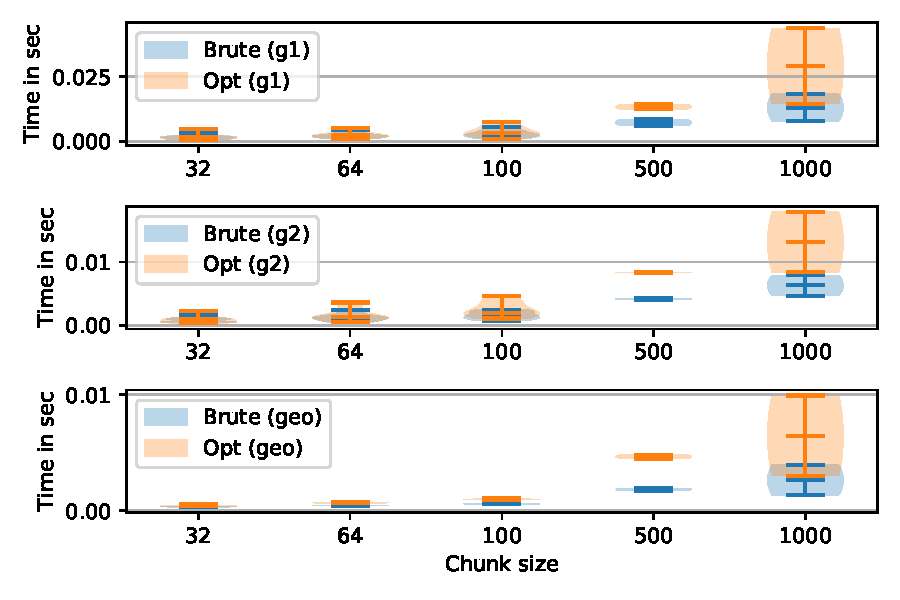
\includegraphics[width=0.5\textwidth]{data/raw/core.pdf}
\caption{Performance of \textit{core} graph querying}
\label{fig:python_core_all}
\end{figure}

\begin{figure}[h]
\centering
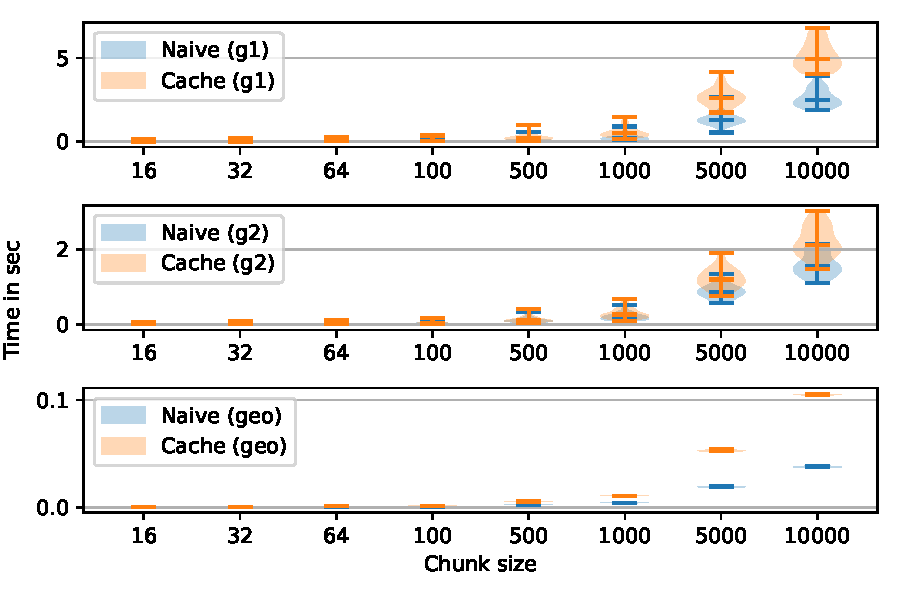
\includegraphics[width=0.5\textwidth]{data/raw/go.pdf}
\caption{Performance of \textit{go} graph querying}
\label{fig:python_go_all}
\end{figure}

\begin{figure}[h]
\centering
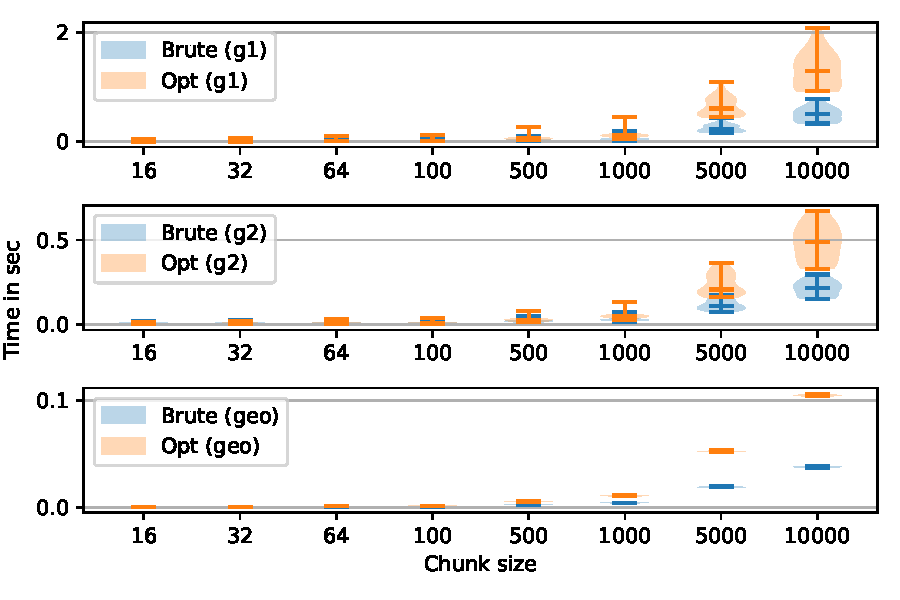
\includegraphics[width=0.5\textwidth]{data/raw/eclass_514en.pdf}
\caption{Performance of \textit{eclass\_514en} graph querying}
\label{fig:python_eclass_all}
\end{figure}

\begin{figure}[h]
\centering
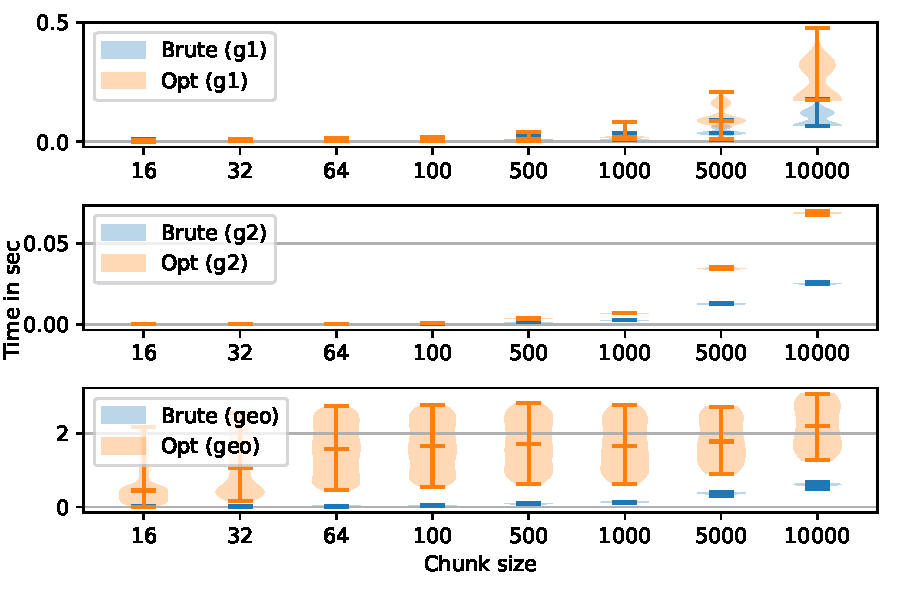
\includegraphics[width=0.5\textwidth]{data/raw/geospecies.pdf}
\caption{Performance of \textit{geospecies} graph querying}
\label{fig:python_geospecies_all}
\end{figure}

\begin{figure}[h]
\centering
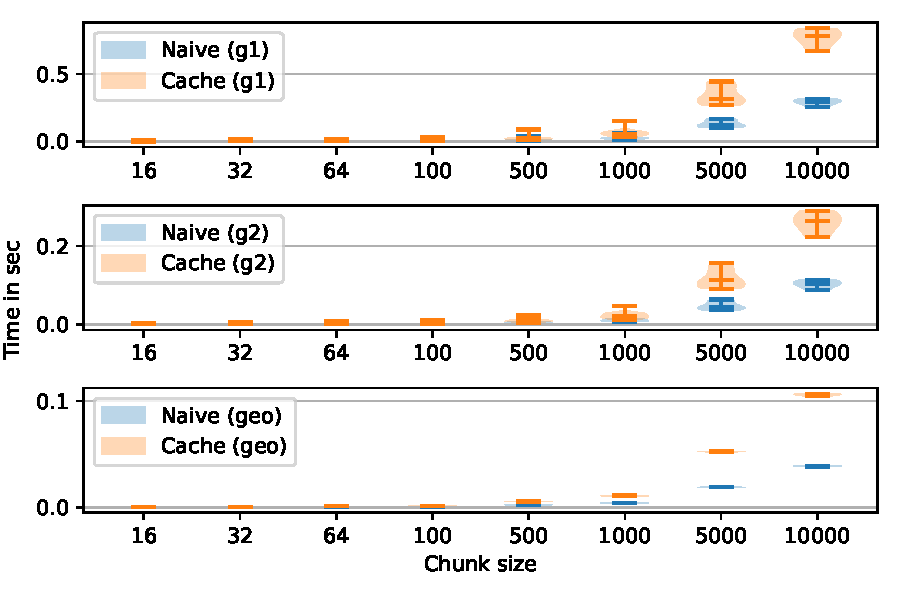
\includegraphics[width=0.5\textwidth]{data/raw/enzyme.pdf}
\caption{Performance of \textit{enzyme} graph querying}
\label{fig:python_enzyme_all}
\end{figure}

\begin{figure}[h]
\centering
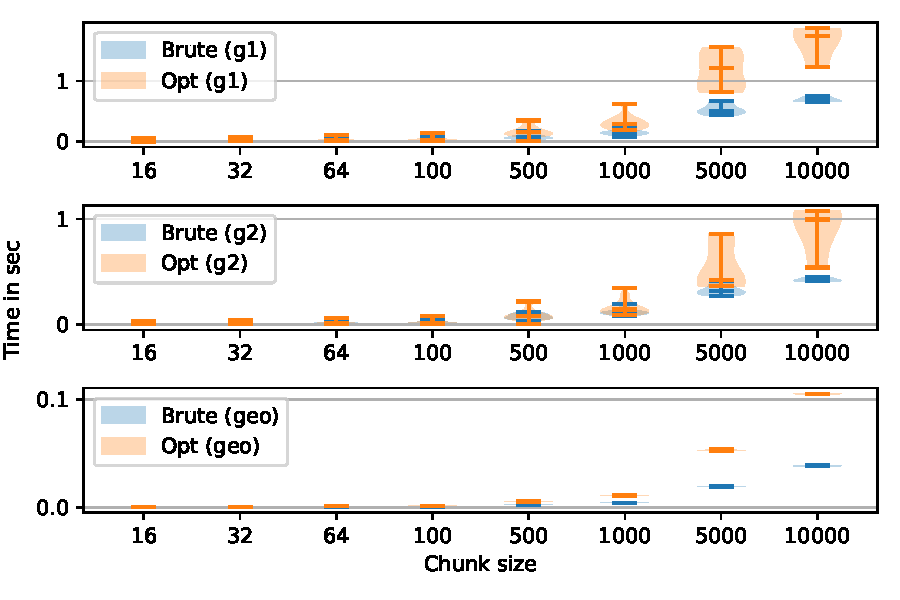
\includegraphics[width=0.5\textwidth]{data/raw/gohierarchy.pdf}
\caption{Performance of \textit{gohierarchy} graph querying}
\label{fig:python_gohierarchy_all}
\end{figure}


\begin{figure}[h]
\centering
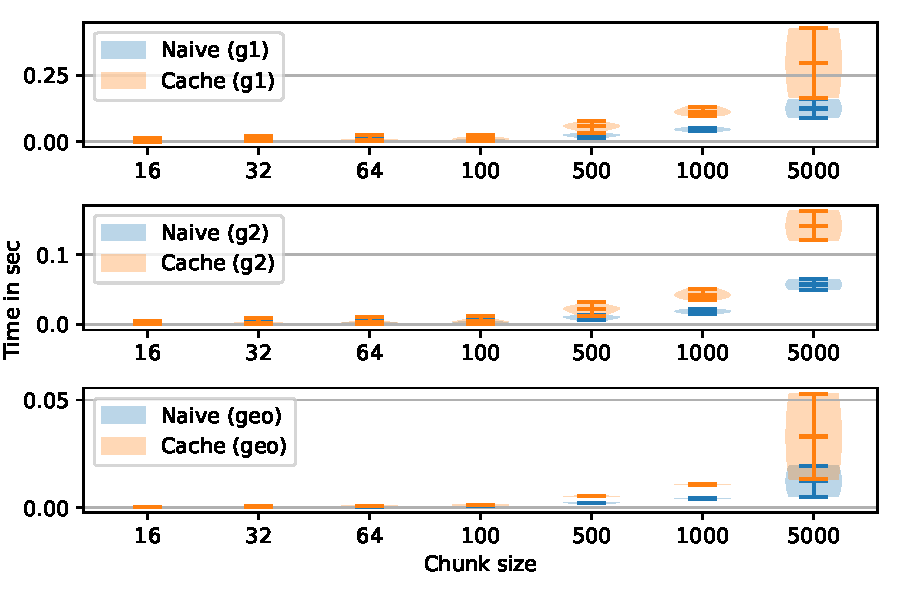
\includegraphics[width=0.5\textwidth]{data/raw/pathways.pdf}
\caption{Performance of \textit{pathways} graph querying}
\label{fig:python_pathways_all}
\end{figure}

\begin{figure}[h]
\centering
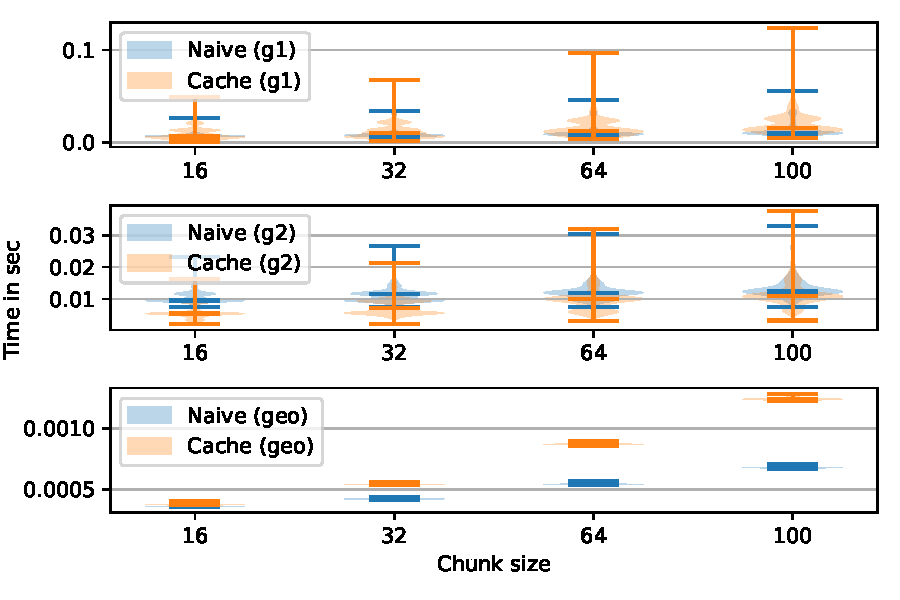
\includegraphics[width=0.5\textwidth]{data/raw/eclass_514en_4.pdf}
\caption{Performance of \textit{eclass\_514en} graph querying with small chunks}
\label{fig:python_eclass_small}
\end{figure}

\begin{figure}[h]
\centering
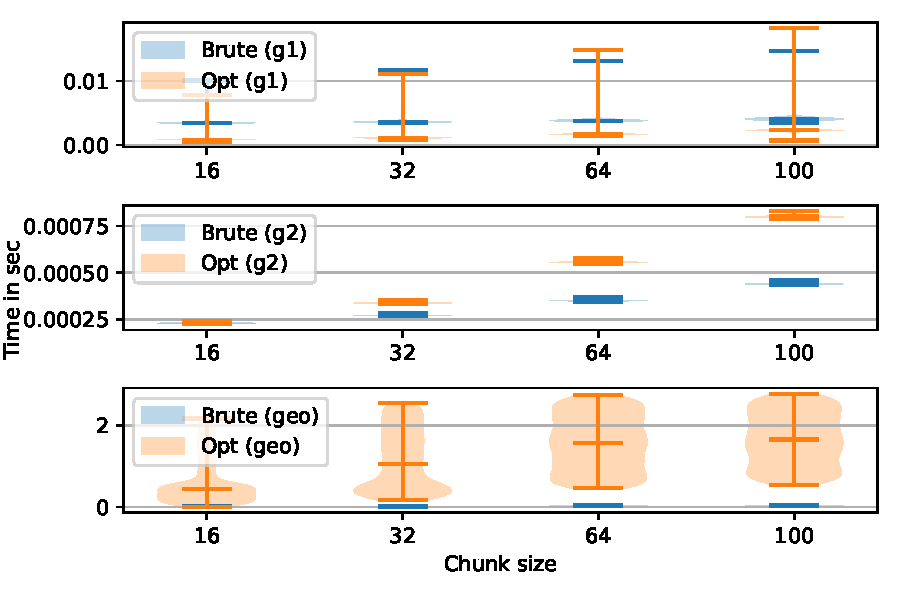
\includegraphics[width=0.5\textwidth]{data/raw/geospecies_4.pdf}
\caption{Performance of \textit{geospecies} graph querying with small chunks}
\label{fig:python_geospecies_small}
\end{figure}

\begin{figure}[h]
\centering
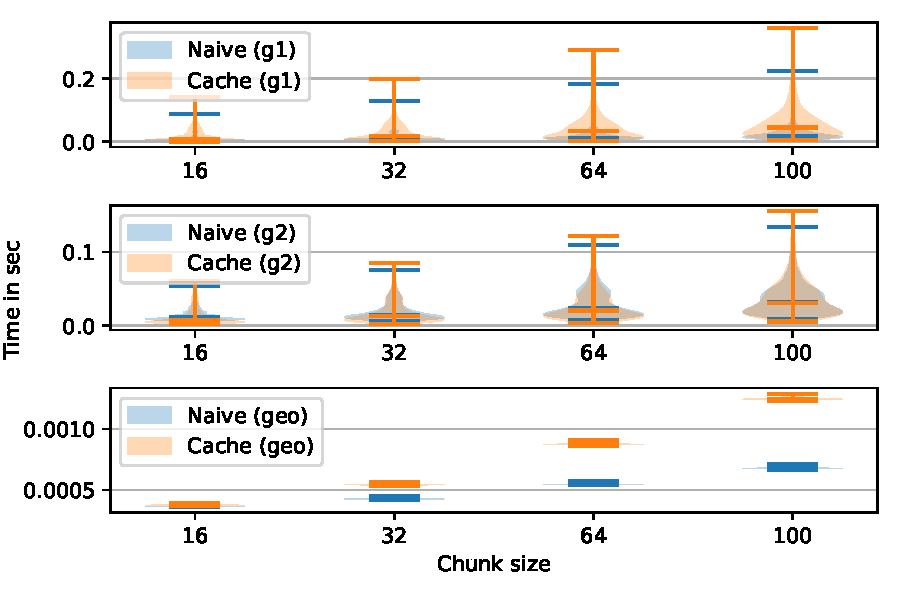
\includegraphics[width=0.5\textwidth]{data/raw/go_4.pdf}
\caption{Performance of \textit{go} graph querying with small chunks}
\label{fig:python_go_small}
\end{figure}


First of all, we can see that even for the cases when the input graph does not contain edges used in a query, the chunk processing time grows with the size of the chunk.
For example, consider the results for \textit{geo} query for all graphs except \textit{geospecies} and \textit{enzyme}.
Thus, the preliminary check of the existence of the edges of interest may improve performance.

We can also see, that the chunk processing time significantly depends on the graph structure.
For example, \textit{go} graph querying requires more than 5 seconds (fig.~\ref{fig:python_go_all}), while \textit{geospecies} graph querying requires less than 0.5 seconds (fig.~\ref{fig:python_geospecies_all}) for the chunks of size 10~000 and the query $g_1$,.

The comparison of two versions of the algorithm shows that the algorithm without caching is significantly faster in almost all cases, even when the graph does not contain edges of interest.
Analysis of results for small chunks (fig.~\ref{fig:python_eclass_small}--\ref{fig:python_go_small}) shows that it is always true.
For example, median time for algorithm with caching is slightly better than for the naive version for \textit{eclass\_514en} graph and query $g_2$ (fig.~\ref{fig:python_geospecies_small}).
On the other hand, algorithm with caching is drastically slower than the naive version for \textit{geospecies} graph and $geo$ query (fig.\ref{fig:python_geospecies_small}).
At the same time, for \textit{go} graph and $g_2$ query, median time of both versions is comparable, while time for the worst queries is better for the naive version.
Moreover, caching requires additional memory in comparison with the naive version of the algorithm.
Thus we conclude, that the query results caching introduces significant overhead and does not lead to significant performance improvements.
We can also conclude that small chunk processing using the naive version is fast enough: the worst time in our experiments is about 0.2 seconds (fig.~\ref{fig:python_go_small}, query $G_1$).


As a result, we conclude that caching is not useful for multiple-source CFPQ for the evaluated cases even if one wants to process several chunks sequentially, or even process full graph chunk-by-chunk.
Thus, we believe that the naive version of the algorithm is better for implementation in a real-world graph database.



